\documentclass[tikz,border=6pt]{standalone}
\usepackage{tikz}
\usetikzlibrary{arrows.meta,calc,shadows.blur,positioning,fit,backgrounds}

% ---------- Color palette (tuned to your image) ----------
\definecolor{silsoBlue}{RGB}{43,92,168}
\definecolor{snRed}{RGB}{232,54,35}
\definecolor{methGray}{RGB}{150,150,150}
\definecolor{gnYellow}{RGB}{240,190,30}
\definecolor{combOrange}{RGB}{225,140,50}
\definecolor{axisGray}{RGB}{80,80,80}

% ---------- Styles ----------
\tikzset{
  laneArrow/.style = {line width=2.8pt, -{Latex[length=6mm,width=3.4mm]}},
  blueLane/.style = {laneArrow, draw=silsoBlue},
  redLane/.style  = {laneArrow, draw=snRed},
  grayLane/.style = {laneArrow, draw=methGray},
  yelLane/.style  = {laneArrow, draw=gnYellow},
  tick/.style = {axisGray, line width=2.2pt},
  year/.style = {axisGray, font=\bfseries\large},
  labelL/.style = {axisGray, font=\bfseries\Large, anchor=east},
  bubbleText/.style = {axisGray, font=\bfseries\footnotesize, align=center},
  laneNote/.style = {axisGray, font=\bfseries\scriptsize, align=left}
}

% ---------- Teardrop milestone helper ----------
\newdimen\tdSize
\newdimen\tdTail
\newdimen\tdCtrlX
\newdimen\tdCtrlY
\newdimen\tdText
\newcounter{tdBubble}

% \teardrop{x}{y}{color}{diameter}{text}
\newcommand{\teardrop}[5]{%
  \stepcounter{tdBubble}%
  \tdSize=#4\relax
  \tdTail=.58\tdSize
  \tdCtrlX=.26\tdSize
  \tdCtrlY=.14\tdSize
  \tdText=.72\tdSize
  \edef\tdName{td\arabic{tdBubble}}%
  \node[draw=#3, line width=2.6pt, fill=white,
    blur shadow={shadow blur steps=5,shadow blur extra rounding=1.2pt},
    minimum width=#4, minimum height=#4, circle, inner sep=6pt]
    (\tdName) at (#1,#2) {\strut\parbox{\the\tdText}{\centering \textcolor{black}{#5}}\strut};
  \coordinate (\tdName-tip) at ($(\tdName.east)+(\tdTail,0)$);
  \begin{scope}[on background layer]
    \draw[#3, line width=2.6pt, fill=white]
      (\tdName.east)
        .. controls +(\tdCtrlX,\tdCtrlY) .. (\tdName-tip)
        .. controls +(-\tdCtrlX,-\tdCtrlY) .. (\tdName.east)
        -- cycle;
  \end{scope}%
}

\begin{document}
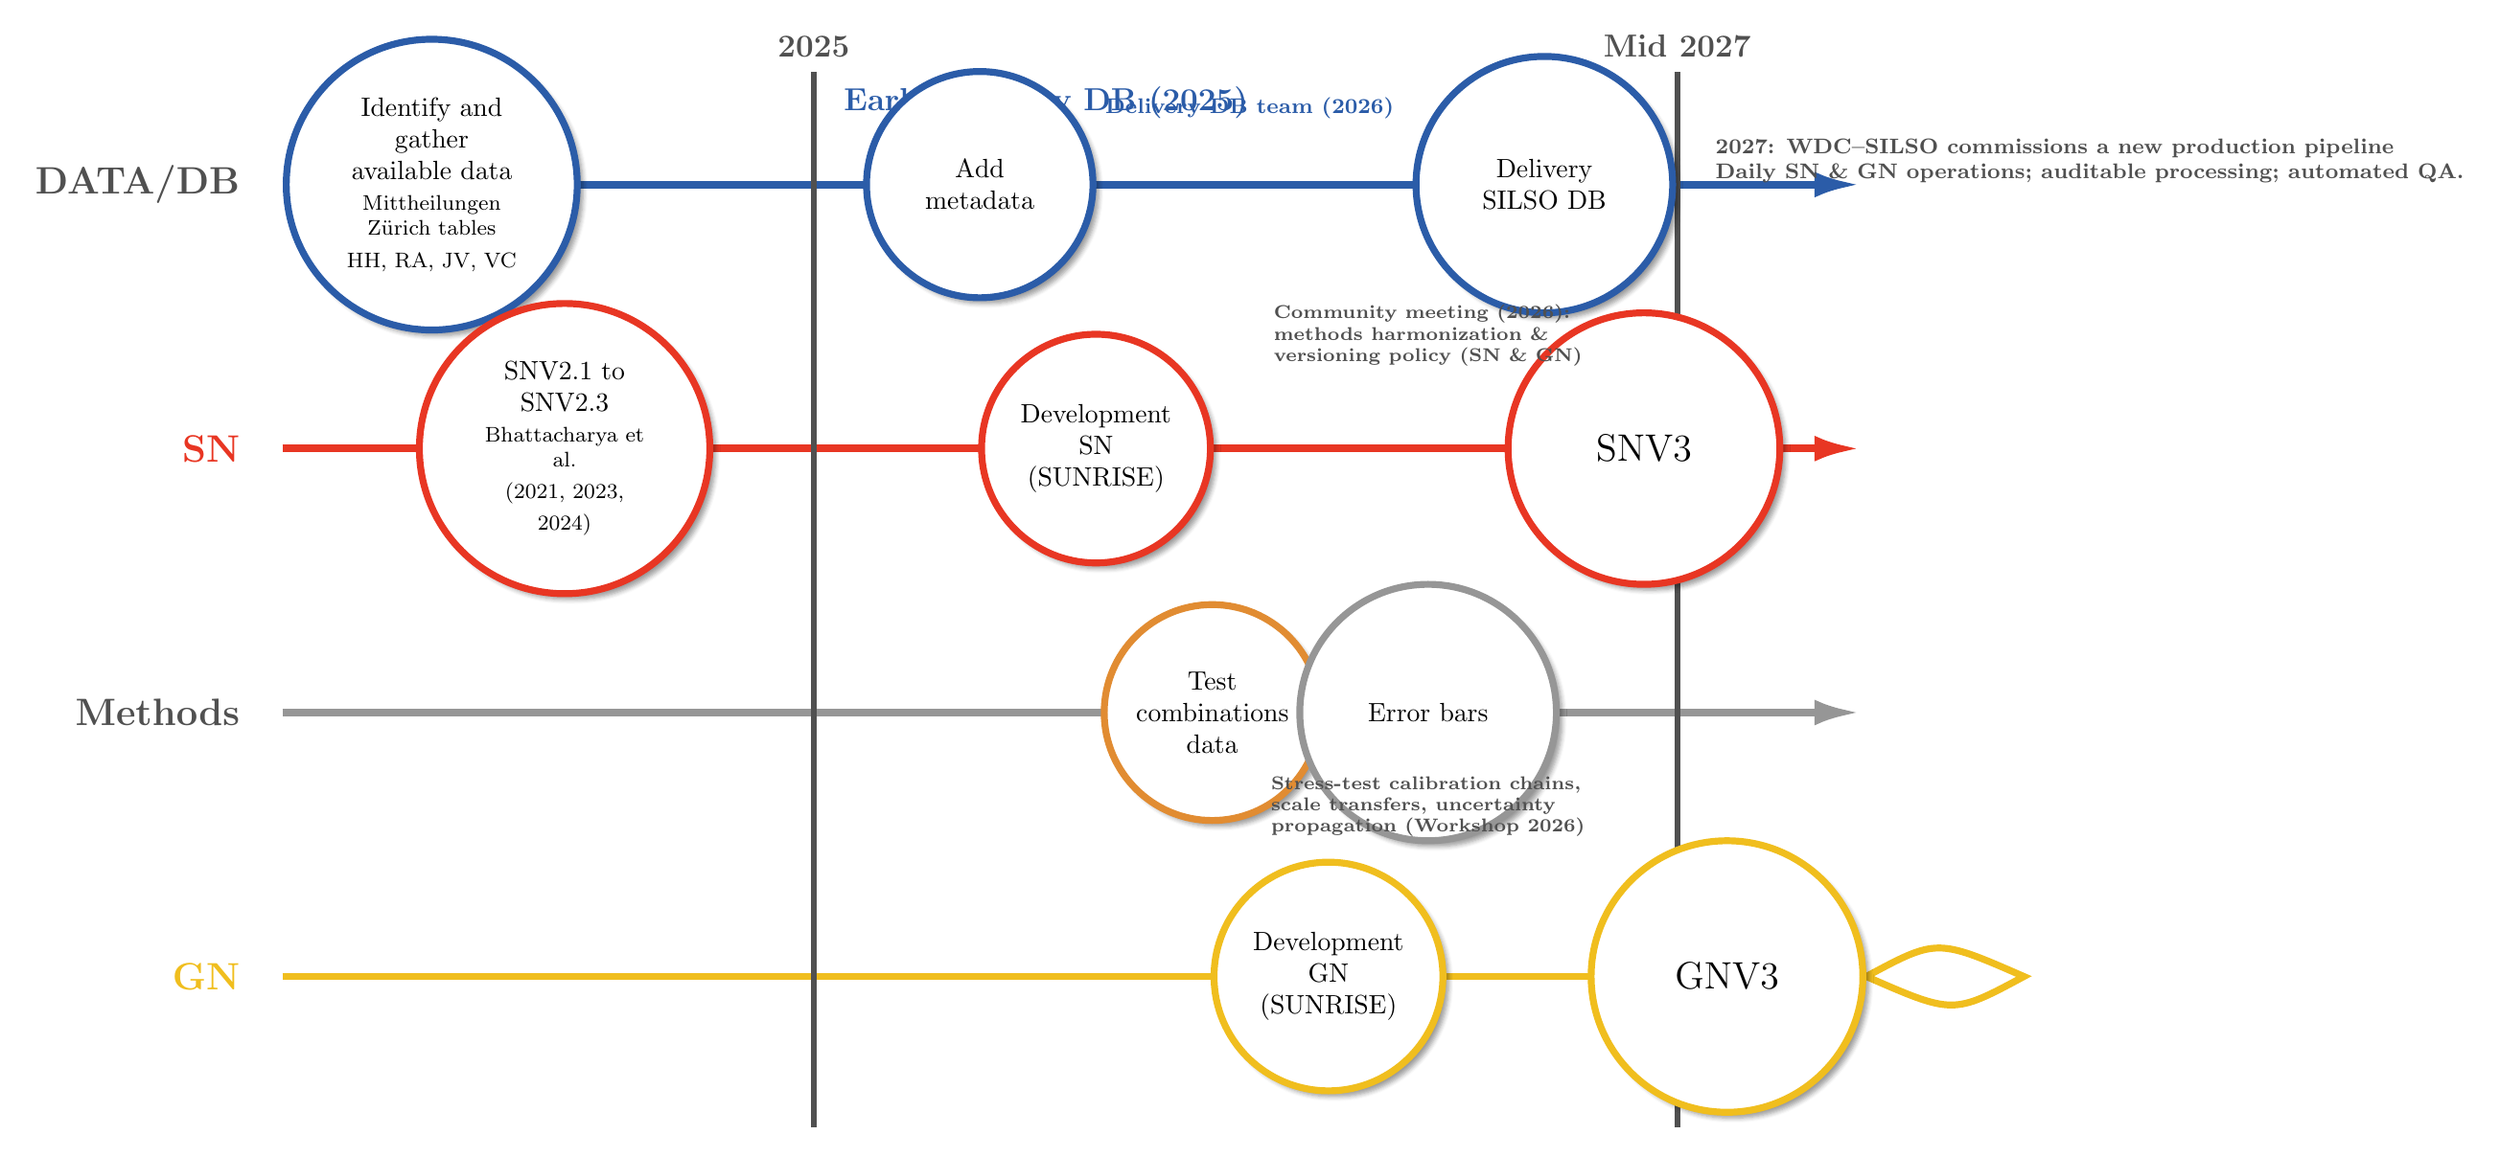
\begin{tikzpicture}[x=1.1cm,y=1.25cm]

% Geometry / coordinates
\def\xmin{0}
\def\xmax{19.0}
\def\xTickA{6.4}
\def\xTickB{16.8}
\def\laneStart{4}
\def\laneGap{2.8} % increased to add more vertical spacing between timelines
\def\laneDB{\laneStart}
\def\laneSN{\laneStart-\laneGap}
\def\laneME{\laneSN-\laneGap}
\def\laneGN{\laneME-\laneGap}

% Lane labels (left)
\node[labelL] at (\xmin-0.4,\laneDB) {DATA/DB};
\node[labelL, text=snRed] at (\xmin-0.4,\laneSN) {SN};
\node[labelL] at (\xmin-0.4,\laneME) {Methods};
\node[labelL, text=gnYellow] at (\xmin-0.4,\laneGN) {GN};

% Lanes (long arrows)
\draw[blueLane] (\xmin,\laneDB) -- (\xmax,\laneDB);
\draw[redLane]  (\xmin,\laneSN) -- (\xmax,\laneSN);
\draw[grayLane] (\xmin,\laneME) -- (\xmax,\laneME);
\draw[yelLane]  (\xmin,\laneGN) -- (\xmax,\laneGN);

% Time ticks
\draw[tick] (\xTickA,\laneGN-1.6) -- (\xTickA,\laneDB+1.2);
\node[year, anchor=south] at (\xTickA,\laneDB+1.25) {2025};

\draw[tick] (\xTickB,\laneGN-1.6) -- (\xTickB,\laneDB+1.2);
\node[year, anchor=south] at (\xTickB,\laneDB+1.25) {Mid 2027};

% ---------- Milestones / “bubbles” ----------
% Left group (pre-2025)
\teardrop{1.8}{\laneDB}{silsoBlue}{3.2cm}{Identify and gather\\available data\\[2pt]
\footnotesize Mittheilungen\\Zürich tables\\HH, RA, JV, VC}

\teardrop{3.4}{\laneSN}{snRed}{3.2cm}{SNV2.1 to\\SNV2.3\\[2pt]
\footnotesize Bhattacharya et al.\\(2021, 2023, 2024)}

% 2025 callout on DB lane
\node[bubbleText, text=silsoBlue, anchor=south west] at (\xTickA+0.25,\laneDB+0.6)
{\large\bfseries Early Delivery DB (2025)};

% Central development stage (around 2026)
\teardrop{8.4}{\laneDB}{silsoBlue}{3.0cm}{Add metadata}

\teardrop{9.8}{\laneSN}{snRed}{3.0cm}{Development\\SN (SUNRISE)}

\teardrop{11.2}{\laneME}{combOrange}{2.8cm}{Test\\combinations\\data}

\teardrop{12.6}{\laneGN}{gnYellow}{3.0cm}{Development\\GN (SUNRISE)}

% Methods uncertainty block
\teardrop{13.8}{\laneME}{methGray}{3.4cm}{Error bars}

% Right-side deliveries near 2027
\teardrop{15.2}{\laneDB}{silsoBlue}{3.4cm}{Delivery\\SILSO DB}

\teardrop{16.4}{\laneSN}{snRed}{3.6cm}{{\Large SNV3}}

\teardrop{17.4}{\laneGN}{gnYellow}{3.6cm}{{\Large GNV3}}

% ---------- Inline subtitles / ribbons ----------
% DB ribbon text across top lane
\node[bubbleText, text=silsoBlue, anchor=south west] at (9.8,\laneDB+0.6)
{\bfseries Delivery DB team (2026)};

% Small contextual notes above/below lanes
\node[laneNote] at (13.8,\laneSN+1.2) {Community meeting (2026):\\methods harmonization \&\\versioning policy (SN \& GN)};
\node[laneNote] at (13.8,\laneME-1.0) {Stress-test calibration chains,\\scale transfers, uncertainty\\propagation (Workshop 2026)};

% Right-most production note near 2027
\node[bubbleText, align=left, anchor=west] at (\xTickB+0.35,\laneDB+0.25) {%
\textbf{2027:} WDC--SILSO commissions a new production pipeline\\
Daily SN \& GN operations; auditable processing; automated QA.};

\end{tikzpicture}
\end{document}
